% !TEX root =  ../../master.tex
\section{Docker-Netzwerk}

Um eine Basis für die Implementierung der Software zu schaffen und gleichzeitig diese für eine Bereitstellung auf einer Zielumgebung vorzubereiten, wurde sich dazu entschlossen Docker zu verwenden (siehe Kapitel \ref{sec:grundlagen:docker}). 
Die Software selbst besteht aus den Komponenten:
\begin{itemize}
	\item \emph{Front-End}, welches die grafische Benutzeroberfläche der Software bereitstellt,
	\item \emph{Back-End}, welches die die Anbindung zur Datenbank bereitstellt,
	\item \emph{PostgreSQL}, welches zur Speicherung der Daten in Form einer Datenbank dient,
	\item \emph{pgAdmin}, welches eine grafische Benutzeroberfläche zur Datenbankverwaltung bietet.
\end{itemize}

All diese Komponenten können entsprechend dem Microservice-Ansatz (siehe Kapitel \ref{sec:grundlagen:microservices}) unabhängig voneinander arbeiten und bereitgestellt werden. 
Aus diesem Grund lag die Entscheidung nahe, dass jede Komponente in einen eigenen Docker-Container betrieben wird.
Um diese Container entsprechend zu verwalten, kommt Docker-Compose zum Einsatz.
Mit Hilfe von Docker-Compose ist es möglich ein isoliertes Docker-Netzwerk aufzubauen, in dem eine Multi-Container-Anwendung, wie es in diesem Projekt vorgesehen ist, betrieben werden kann.
Die Konfiguration des Netzwerkes für Docker-Compose erfolgt dabei in einer Datei im YAML-Format, welches von Docker vorgegeben wird.

Abbildung \ref{fig:implementierung:docker} zeigt den Aufbau des kompletten Netzwerkes bzw. der Multi-Container-Anwendung mit allen möglichen Komponenten und deren Kommunikationsports. 
Zusätzlich sind die Nutzer (Entwickler und Client), die extern auf die Software zugreifen, ebenfalls dargestellt.

\begin{figure}[H]
	\centering
	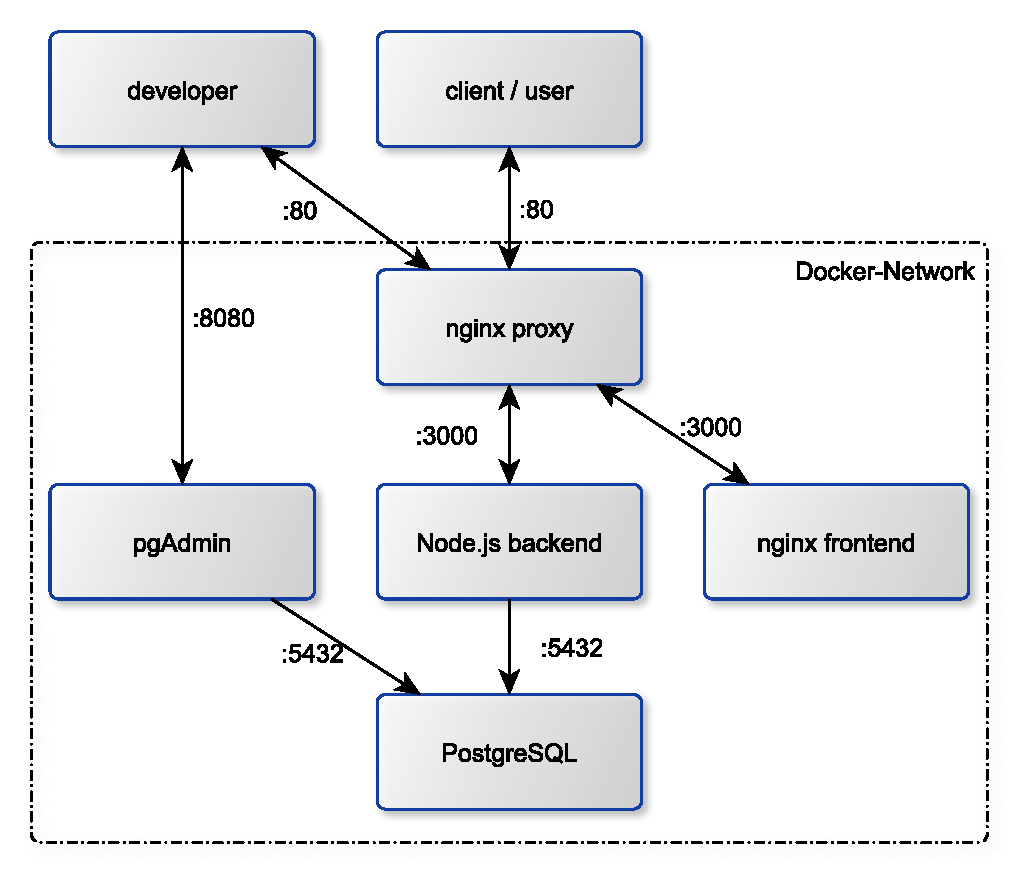
\includegraphics[width=0.75\textwidth]{img/implementierung/network.pdf}
	\captionsetup{justification=centering, format=plain}
	\caption[Docker-Netzwerk-Aufbau]{Docker-Netzwerk-Aufbau \\Quelle: Eigene Darstellung}
	\label{fig:implementierung:docker}
\end{figure}

Die vier Komponenten werden wie dargestellt als einzelne Container hochgefahren und sind von der Außenwelt isoliert. 
Das Back-End wird dabei von einem Node.js-Server und das Front-End von einem nginx-Webserver bereitgestellt.
Damit diese Komponenten überhaupt innerhalb eines Containers betrieben werden können, ist es nötig für jede Komponente eigenes Dockerfile zu schreiben.
Ein Dockerfile ist dabei eine Textdatei, welche eine Bauanleitung eines Container-Images darstellt.
Auf Basis dieser Container-Images werden beim Hochfahren des Netzwerkes durch Docker-Compose die entsprechenden Container erstellt.

Um das Front- und Back-End zusätzlich von der Außenwelt abzukapseln und einen konsistenten Zugriff über die selbe Schnittstelle auf die Softwarezu gewährleisten, ist zusätzlich ein weiterer nginx-Webserver (nginx-Proxy) vor diese Komponenten geschaltet.
Dieser Webserver dient dabei als Proxy, welcher als Vermittler zwischen den genannten Komponenten und der Außenwelt dient.
Dementsprechend erfolgt der Zugriff zur Software einzig und allein über diesen Proxy, da nur dessen Port (80) an das Hostsystem freigegeben wird.
Für den Entwickler und den Administrator des Systems existiert zusätzlich noch die Möglichkeit über Port 8080 auf den pgAdmin-Container zuzugreifen. 
Im späteren Live-Betrieb sollte der Zugang zu pgAdmin jedoch ebenfalls eingeschränkt werden.

Da im Entwicklungsbetrieb immer nur bestimmte Container benötigt werden, ist es nötig mehrere Konfigurationsdateien für Docker-Compose anzulegen.
Dementsprechend wird für die Back-End-Entwicklung nur der PostgreSQL- und der pgAdmin-Container benötigt.
Für die Front-End-Entwicklung kann zusätzlich der Back-End-Container hochgefahren werden.
